\section{Evaluation}\label{sec:eval}

To evalute feature-sensitive coverages, we apply $\tool$ to the latest language
specification (ES13, 2022)~\cite{es13} with different $k$-FS and $k$-FCPS
node/branch coverages to synthesize JavaScript conformance tests.
%
As a result, we synthesize \inred{185,246} conformance tests using $\tool$ with
five different graph coverage criteria: 1) a node/branch coverage and 2) $1$-FS,
3) $2$-FS, 4) $1$-FCPS, and 5) $2$-FCPS node/branch coverages.
%
Our evaluation platform is a 4.0GHz Intel(R) Core(TM) i7-6700k and 32GB of RAM
(Samsung DDR4 2133MHz 8GB*4), and it takes \inred{72} hours to synthesize
conformance tests.
%
We evaluated the synthesized conformance test suite with the following four
research questions:
\begin{itemize}
  \item \textbf{RQ1 (Conformance Bug Detection):} How many conformance bugs of
    JavaScript engines and transpilers do conformance tests synthesized by
    $\tool$ detect? (Section~\ref{sec:conform-bug})
  \item \textbf{RQ2 (Impact of $k$-FS Coverages):} What effect do $k$-FS
    coverages have in detecting conformance bugs?
    (Section~\ref{sec:impact-k-fs})
  \item \textbf{RQ3 (Impact of $k$-FCPS Coverages):} What effect do $k$-FCPS
    coverages have in detecting conformance bugs compared to $k$-FS coverages?
    (Section~\ref{sec:impact-k-fcps})
  \item \textbf{RQ4 (Comparison with Test262):} Could conformance tests
    synthesized by $\tool$ improve Test262, the official JavaScript conformance
    suite maintained by hand? (Section~\ref{sec:compare-test262})
\end{itemize}

%----------------------------------------%
%----------------------------------------%

\subsection{Conformance Bug Detection}\label{sec:conform-bug}

\begin{table}
\caption{
  Detected conformance bugs in JavaScript engines and transpilers.
}
\vspace*{-.5em}
{
\small
\label{tab:conform-bugs}
\begin{tabular}{?c?l|l|l?r|r|r?}
\toprule\\[-1.6em]

\multicolumn{1}{?c?}{\multirow{2}{*}{\textbf{Kind}}}
& \multicolumn{1}{c|}{\multirow{2}{*}{\textbf{Name}}}
& \multicolumn{1}{c|}{\multirow{2}{*}{\textbf{Version}}}
& \multicolumn{1}{c?}{\multirow{2}{*}{\textbf{Release}}}
& \multicolumn{3}{c?}{\textbf{\# Detected Unique Bugs}} \\\cline{5-7}

&&&
& \multicolumn{1}{c|}{\textbf{\# New}}
& \multicolumn{1}{c|}{\textbf{\# Confirmed}}
& \multicolumn{1}{c?}{\textbf{\# Reported}}\\

\toprule\\[-1.6em]

\multirow{5}{*}{Engine}
& V8            & v10.8.121 & 2022.10.06 & \x{0} & \x{0} & \x{3} \\\cline{2-7}
& JSC           & v615.1.10 & 2022.10.26 & \x{4} & \x{4} & \x{14}\\\cline{2-7}
& GrallJS       & v22.2.0   & 2022.07.26 & \x{7} & \x{7} & \x{9} \\\cline{2-7}
& SpiderMonkey  & v107.0    & 2022.10.24 & \x{1} & \x{3} & \x{3} \\\cline{2-7}
& \multicolumn{3}{c?}{\textbf{Total}}    & \y{12}& \y{14}& \y{29}\\

\toprule\\[-1.6em]

\multirow{5}{*}{Transpiler}
& Babel         & v7.19.1   & 2022.09.15 & \x{33}& \x{33}& \x{39}\\\cline{2-7}
& SWC           & v1.3.10   & 2022.10.21 & \x{30}& \x{30}& \x{32}\\\cline{2-7}
& Terser        & v5.15.1   & 2022.10.05 & \x{1} & \x{1} & \x{15}\\\cline{2-7}
& Obfuscator    & v4.0.0    & 2022.02.15 & \x{0} & \x{0} & \x{3} \\\cline{2-7}
& \multicolumn{3}{c?}{\textbf{Total}}    & \y{64}& \y{64}& \y{89}\\

\toprule\multicolumn{1}{c}{}\\[-1.6em]


\multicolumn{4}{?c?}{\textbf{Total}}
& \y{76}& \y{78}& \y{118}\\

\toprule\multicolumn{1}{c}{}\\[-1.6em]
\end{tabular}
}
\end{table}

%----------------------------------------%

Using the synthesized JavaScript conformance tests, we check the conformance of
eight mainstream tools (four engines and four transpilers) listed in
Table~\ref{tab:conform-bugs}.
%
We select them as evaluation targets because they support all the language
features in ES13.
%
V8, JSC, and SpiderMonkey are JavaScript engines used in web browsers, Google
Chrome, Apple Safari, and Mozilla Firefox, respectively.
%
GraalJS is a JavaScript engine built on GraalVM, a JDK distribution developed by
Oracle written for JVM languages along with support for cloud-native and
polyglot.
%
Babel and SWC are transpilers that desugar new language features into old ones,
usually ES5.1 features, for legacy host environments.
%
Terser is a code compressor that reduces the code size by removing code
fragments, making names smaller, or inlining variable references.
%
Finally, JavaScript Obfuscator obfuscates code to make it hard to understand and
reverse-engineering.

%----------------------------------------%

Table~\ref{tab:conform-bugs} gives the distribution of the detected conformance
bugs by \inred{185,246} synthesized conformance tests.
%
We found conformance bugs in all the evaluation targets using the synthesized
conformance tests.
%
In addition, we manually inspected the failed conformance test cases,
categorized them as \inred{118} unique conformance bugs, and reported them to
the developers of the target tools.
%
As a result, \inred{78} out of \inred{118} bugs were officially confirmed, and
\inred{76} were newly discovered bugs.
%
The other \inred{40} reported bugs are still under review, or developers have
not yet responded.
%
Among \inred{118} detected bugs, \inred{29} are engine bugs, and \inred{118} are
transpiler bugs.
%
The two most trusted engines are V8 and SpiderMonkey because they have only three
conformance bugs.
%
Hence, we use V8 as the default engine during the transpiler conformance check.
%
If V8 fails a conformance test, we use another JavaScript engine that passes the
test for the conformance check of a transpiler.
%
Among transpilers, Terser and JavaScript Obfuscator contain only \inred{15} and
\inred{3} bugs, respectively, but Babel and SWC have \inred{39} and
\inred{32} transpiler conformance bugs, respectively.
%
In happens because transpilers desugaring new language features to ES5.1 is a
more challenging than compressing or obfuscating the code.

%----------------------------------------%
%----------------------------------------%

\subsection{Impact of $k$-FS Coverages}\label{sec:impact-k-fs}

\begin{table}
\label{tab:compare}
\caption{
  Comparison of synthesized conformance test suite guided-by five different
  graph coverage criteria: 1) a node/branch coverage, and 2) $1$-FS, 3)
  $2$-FS, 4) $1$-FCPS, and 5) $2$-FCPS node/branch coverages.
}
\vspace*{-.5em}
{
\small
\begin{tabular}{?c?r|r|r?r|r?}
\toprule\\[-1.6em]

\multicolumn{1}{?c?}{\multirow{2}{*}{\textbf{Coverage Criterion}}}
& \multicolumn{3}{c?}{\textbf{\# Covered TRs}}
& \multicolumn{1}{c|}{\multirow{2}{*}{\textbf{\# Syn. Tests}}}
& \multicolumn{1}{c?}{\multirow{2}{*}{\textbf{\# Bugs}}}\\\cline{2-4}

& \multicolumn{1}{c|}{\textbf{\# Nodes (K)}}
& \multicolumn{1}{c|}{\textbf{\# Branchs (K)}}
& \multicolumn{1}{c?}{\textbf{\# Total (K)}}
&&\\

\toprule\\[-1.6em]

Node/Branch
& \x{2.1}     & \x{10.0}    & \x{12.1}    & \x{2,095} & \x{45}  \\\hline
$1$-FS Node/Branch
& \x{61.5}    & \x{34.2}    & \x{95.7}    & \x{5,336} & \x{60}  \\\hline
$1$-FCPS Node/Branch
& \x{257.7}   & \x{133.2}   & \x{390.9}   & \x{5,446} & \x{75}  \\\hline
$2$-FS Node/Branch
& \x{1,131.5} & \x{663.3}   & \x{1,794.8} & \x{83,668}& \x{115} \\\hline
$2$-FCPS Node/Branch
& \x{2,854.9} & \x{1,500.4} & \x{4,355.3} & \x{88,701}& \x{118} \\

\toprule\multicolumn{1}{c}{}\\[-1.6em]

\end{tabular}
}
\end{table}

\todo

%----------------------------------------%
%----------------------------------------%

\subsection{Impact of $k$-FCPS Coverages}\label{sec:impact-k-fcps}

\begin{figure}
  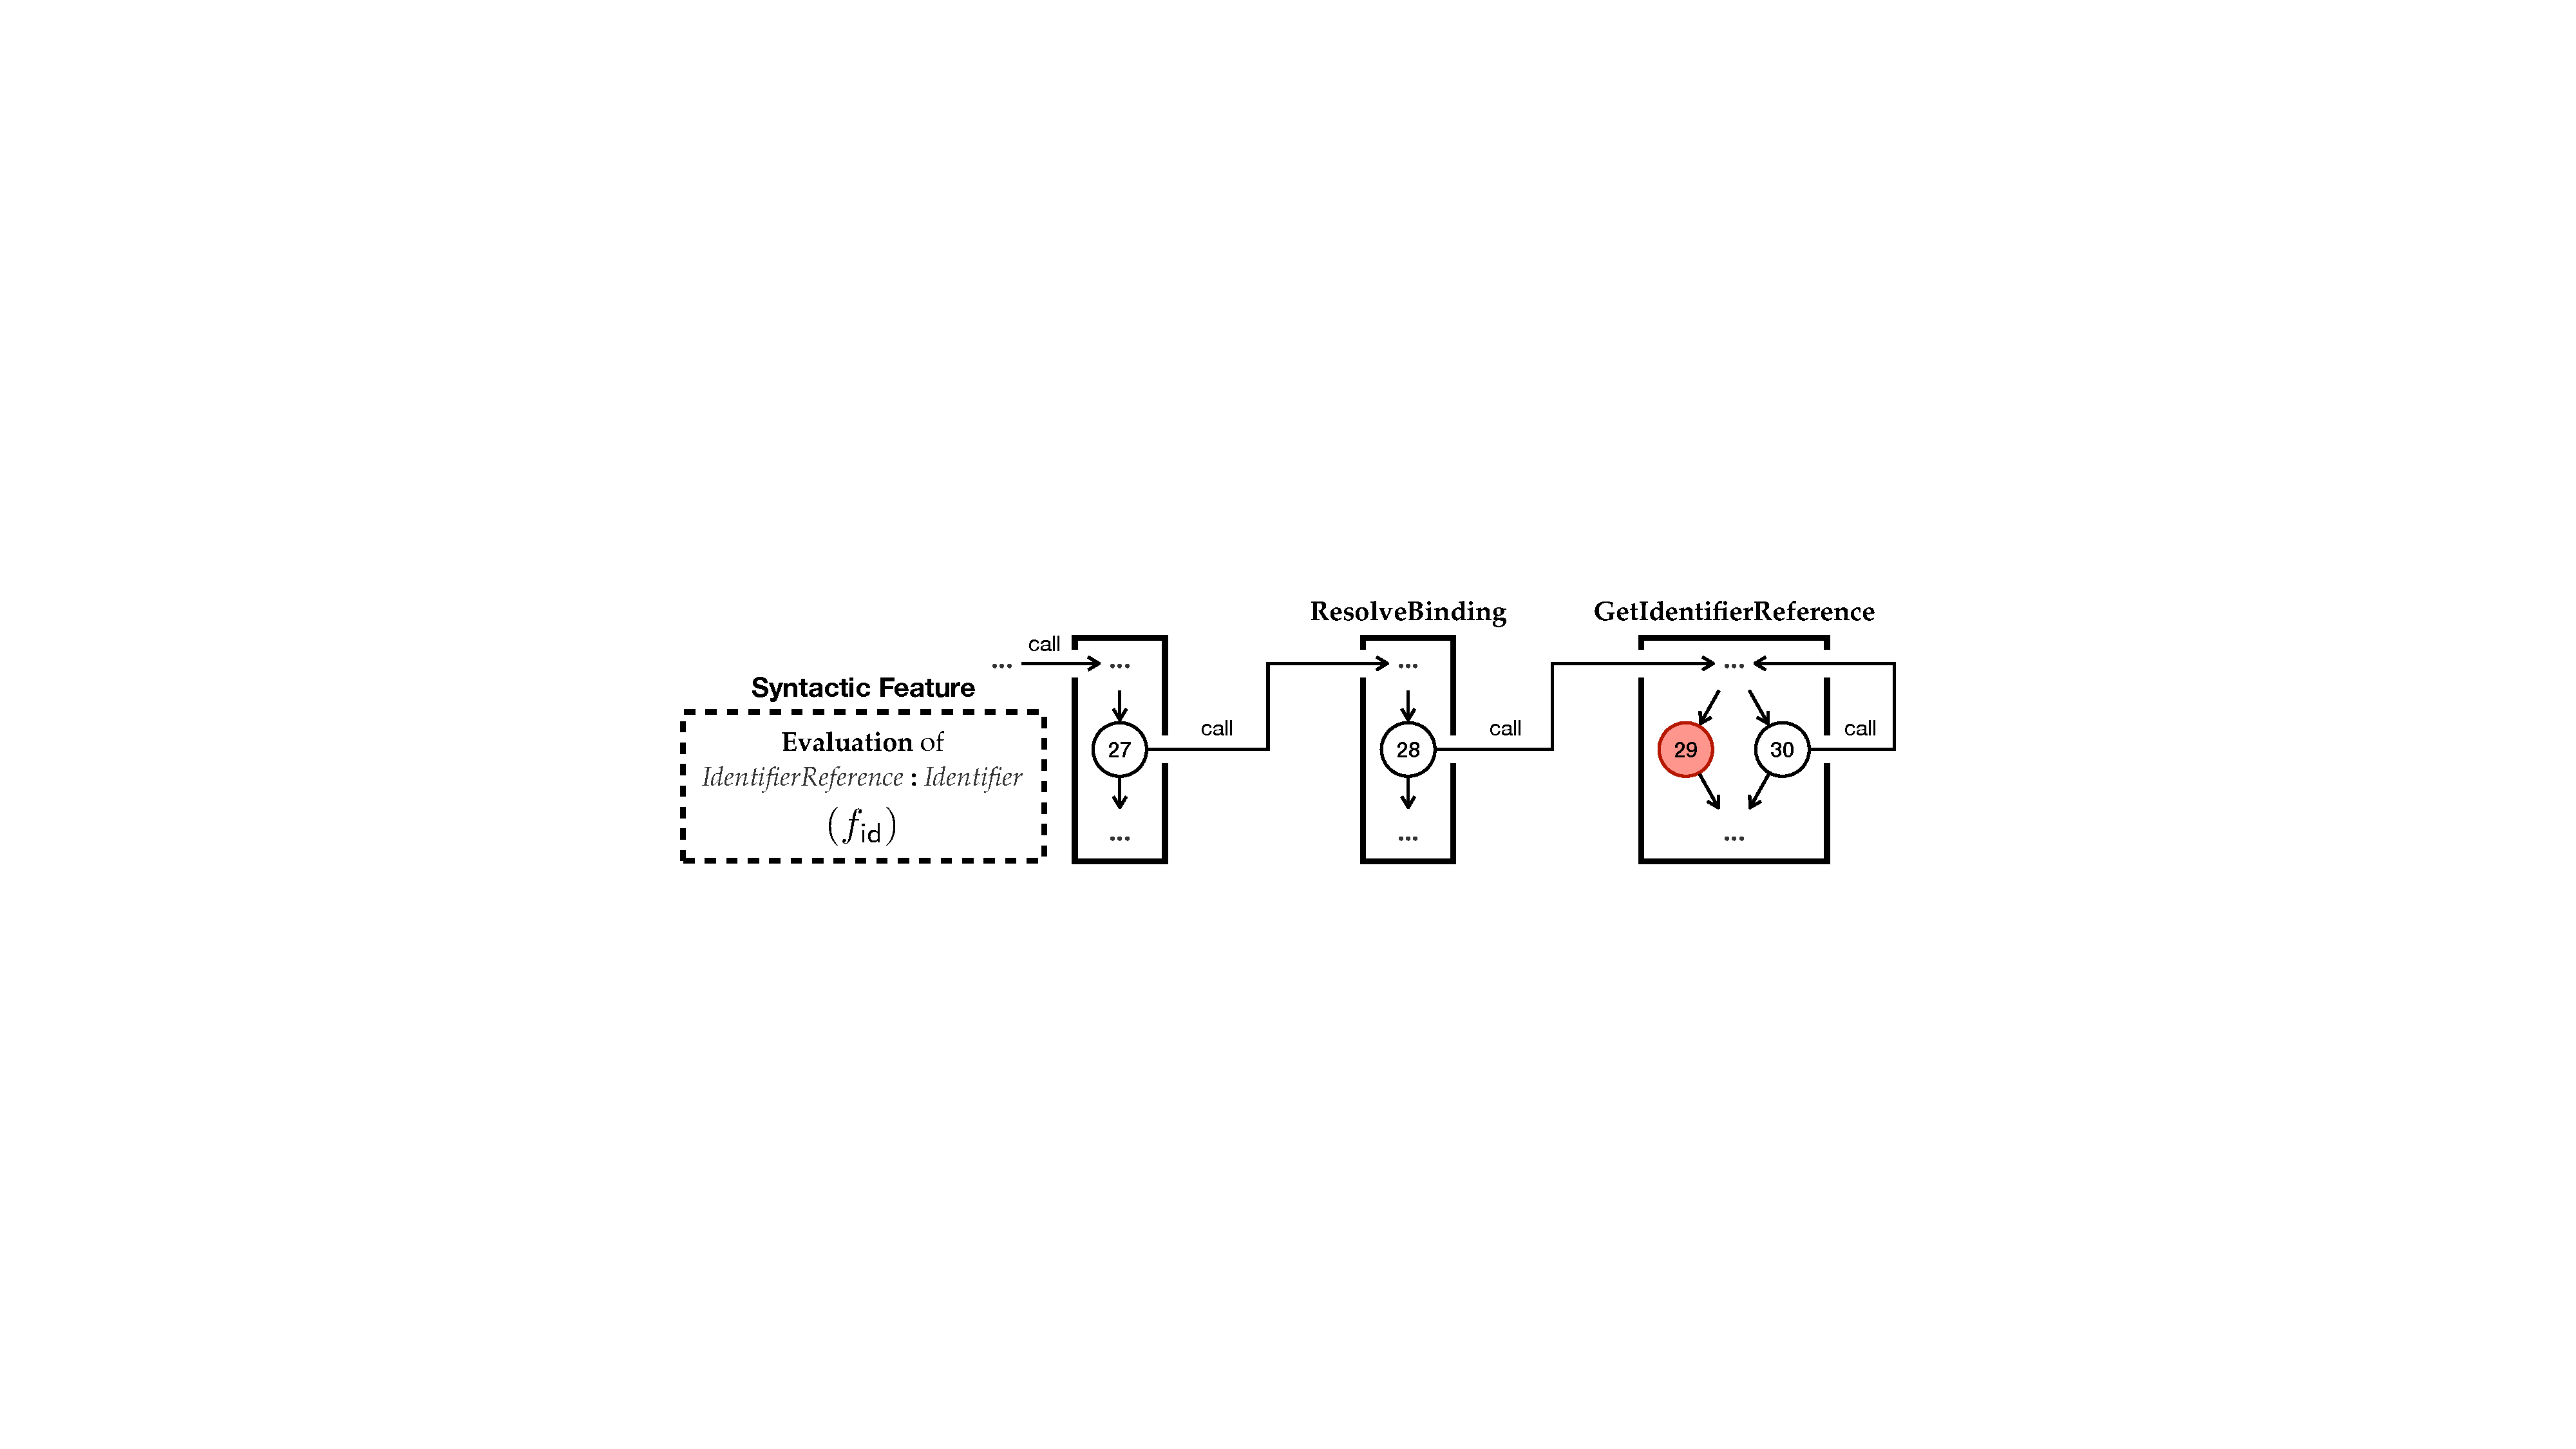
\includegraphics[width=0.85\textwidth]{img/spec-cfg-id}
  \caption{
    .
  }
  \label{fig:spec-cfg-id}
\end{figure}

\todo

%----------------------------------------%
%----------------------------------------%

\subsection{Comparison with Test262}\label{sec:compare-test262}

\todo
